% Interspeech 2025 Presentation: Joint ASR and DID
\documentclass[aspectratio=169,xcolor=dvipsnames]{beamer}
% \documentclass[xcolor=dvipsnames]{beamer}
\usetheme{CambridgeUS}
\usetheme{Antibes}
\usecolortheme{beaver}

\setbeamercolor{structure}{fg=burntumber}
\setbeamercolor*{title}{bg=burntumber,fg=white}
\setbeamercolor{section in head/foot}{bg=burlywood!60}
\setbeamercolor{frametitle}{fg=sienna,bg=burlywood!60}
\setbeamercolor{block body}{bg=burlywood!35}
\setbeamercolor{background canvas}{bg=burlywood!25}
\setbeamercolor{section in head/foot}{fg=black}
\setbeamercolor{normal text}{fg=rosewood}
\setbeamercolor{author in head/foot}{fg=white,bg=mahogany}
\setbeamercolor{block title}{bg=burntumber,fg=white}
\usepackage{color} % This is the package for including colors.
\usepackage{graphics} % This is the package for including the pictures
\usepackage{tikz} % I used this package for including the lab logo on top of every slide
\usepackage[absolute,overlay]{textpos} % This package to insert textblocks
\usepackage{graphicx,tabularx}
\usepackage[table,xcdraw]{xcolor}
\usepackage{multirow}
\usepackage{booktabs}
\usepackage{arydshln}
\usepackage{xcolor}
\usepackage{url,hyperref}
\usepackage[table]{xcolor}   % for cellcolor
\usepackage{array,booktabs}  % nicer tables

% DEFINE COLORS
%dark colors
\definecolor{burntumber}{rgb}{0.54, 0.2, 0.14}
\definecolor{sienna}{rgb}{0.53, 0.18, 0.09} 
\definecolor{rosewood}{rgb}{0.4, 0.0, 0.04}
% light colors
\definecolor{burlywood}{rgb}{0.87, 0.72, 0.53}
\definecolor{mahogany}{rgb}{0.75, 0.25, 0.0}


% Page Numbering in Footer
\setbeamertemplate{footline}{
    \begin{beamercolorbox}[sep=0.5ex,wd=\paperwidth]{title in head/foot}
        \hspace{1em}\textbf{SPIRE LAB, IISc, Bangalore} \hfill \texttt{saurabhk0317@gmail.com, amartyaveer72@gmail.com, prasantag@gmail.com} \hspace{3em} \insertframenumber \hspace{1em}
    \end{beamercolorbox}
}

\setbeamertemplate{title page}{
    \vbox{}
    \vfill
    \begin{center}
        % Title box with background and centered text
        \begin{beamercolorbox}[wd=\textwidth,rounded=true,center]{title}
            \usebeamerfont{title} \inserttitle
        \end{beamercolorbox}
        
        \vspace{4mm} % Adjusted for proper spacing
        
        % Author list with color and proper centering
        {\usebeamercolor[fg]{author}\usebeamerfont{author}
        \textcolor{mahogany}{\insertauthor}}\par
        
        \vspace{4mm} % Reduced gap
        
        % Institute information
        {\usebeamercolor[fg]{institute}\usebeamerfont{institute}
        \textcolor{burntumber}{\insertinstitute}}\par
        
        \vspace{4mm} % Adjusted for better alignment
        
        % Logos centered horizontally
        \begin{minipage}{\textwidth}
            \centering
            \includegraphics[width=1.4cm,height=0.8cm,keepaspectratio]{spire_logo.png} \hspace{3cm}
            \includegraphics[width=1.6cm,height=0.8cm,keepaspectratio]{iisc_logo.png} \hspace{3cm}
            \includegraphics[width=1.6cm,height=0.8cm,keepaspectratio]{ee.png}
        \end{minipage}

        \vspace{6mm}

        % Date (placed after logos)
        {\usebeamercolor[fg]{date}\usebeamerfont{date}\insertdate}\par

        % \vspace{12pt} % Adjust spacing for logos
    \end{center}
    \vfill
}

\usefonttheme{professionalfonts}

% Title Slide
\title{Jointly Improving Dialect Identification and ASR in Indian Languages using Multimodal Feature Fusion}

\author{\textcolor{mahogany}{\textbf{Saurabh Kumar}, Amartyaveer, Prasanta Kumar Ghosh}}
\institute[]{
    \textcolor{burntumber}{SPIRE LAB}\\
    \textcolor{burntumber}{Department of Electrical Engineering}\\
    \textcolor{burntumber}{Indian Institute of Science (IISc), Bangalore, India}
}
\date{Interspeech 2025}

% Section Title Formatting
\AtBeginSection[]
{
\begin{frame}<beamer>
\frametitle{Overview}
\tableofcontents[currentsection]
\end{frame}
}

\begin{document}

%------------------------------------------------------------
% Title Frame
%------------------------------------------------------------
\begin{frame}
    \titlepage
\end{frame}

%------------------------------------------------------------
% Outline Frame
%------------------------------------------------------------
\begin{frame}{Overview}
    \tableofcontents
\end{frame}

%------------------------------------------------------------
% Introduction Section
%------------------------------------------------------------
\section{Introduction}

\begin{frame}{Motivation: The Challenge of Dialectal Variation}
    \begin{itemize}
        \item Automatic Speech Recognition (ASR) and Dialect Identification (DID) are critical for linguistically diverse country like India.
        \item Significant dialectal differences in pronunciation, vocabulary, and grammar pose a major challenge for ASR systems~\cite{Udupa_ASRU2023}.
        \item Accurately identifying a speaker's dialect can allow an ASR system to adapt, mitigating errors and improving performance.
        \item Though DID is similar to language identification (LID), DID is inherently difficult as dialects of the same language share many phonetic and lexical characteristics.
    \end{itemize}
\end{frame}

\begin{frame}{Training--Test Modalities for DID}

% \scriptsize
\begin{columns}[T,totalwidth=\textwidth]

  \column{0.5\textwidth}
  \begin{minipage}[t]{\linewidth}
    \centering
    \resizebox{0.8\linewidth}{!}{%
      \begin{tabular}{@{}lccc@{}}
      \toprule
      \textbf{Train $\downarrow$ / Test $\rightarrow$} & \textbf{Audio} & \textbf{Text} & \textbf{Audio+Text} \\
      \midrule
      \textbf{Audio}      & \textbf{Weaker} & -- & -- \\
      \textbf{Text}       & -- & \textbf{Weaker} & -- \\
      \textbf{Audio+Text} & \textbf{Preferred (this work)} & -- & \textbf{Limited} \\
      \bottomrule
      \end{tabular}
    }

    \vspace{1mm}

    % Bottom: figure (cap the height so content below columns fits)
    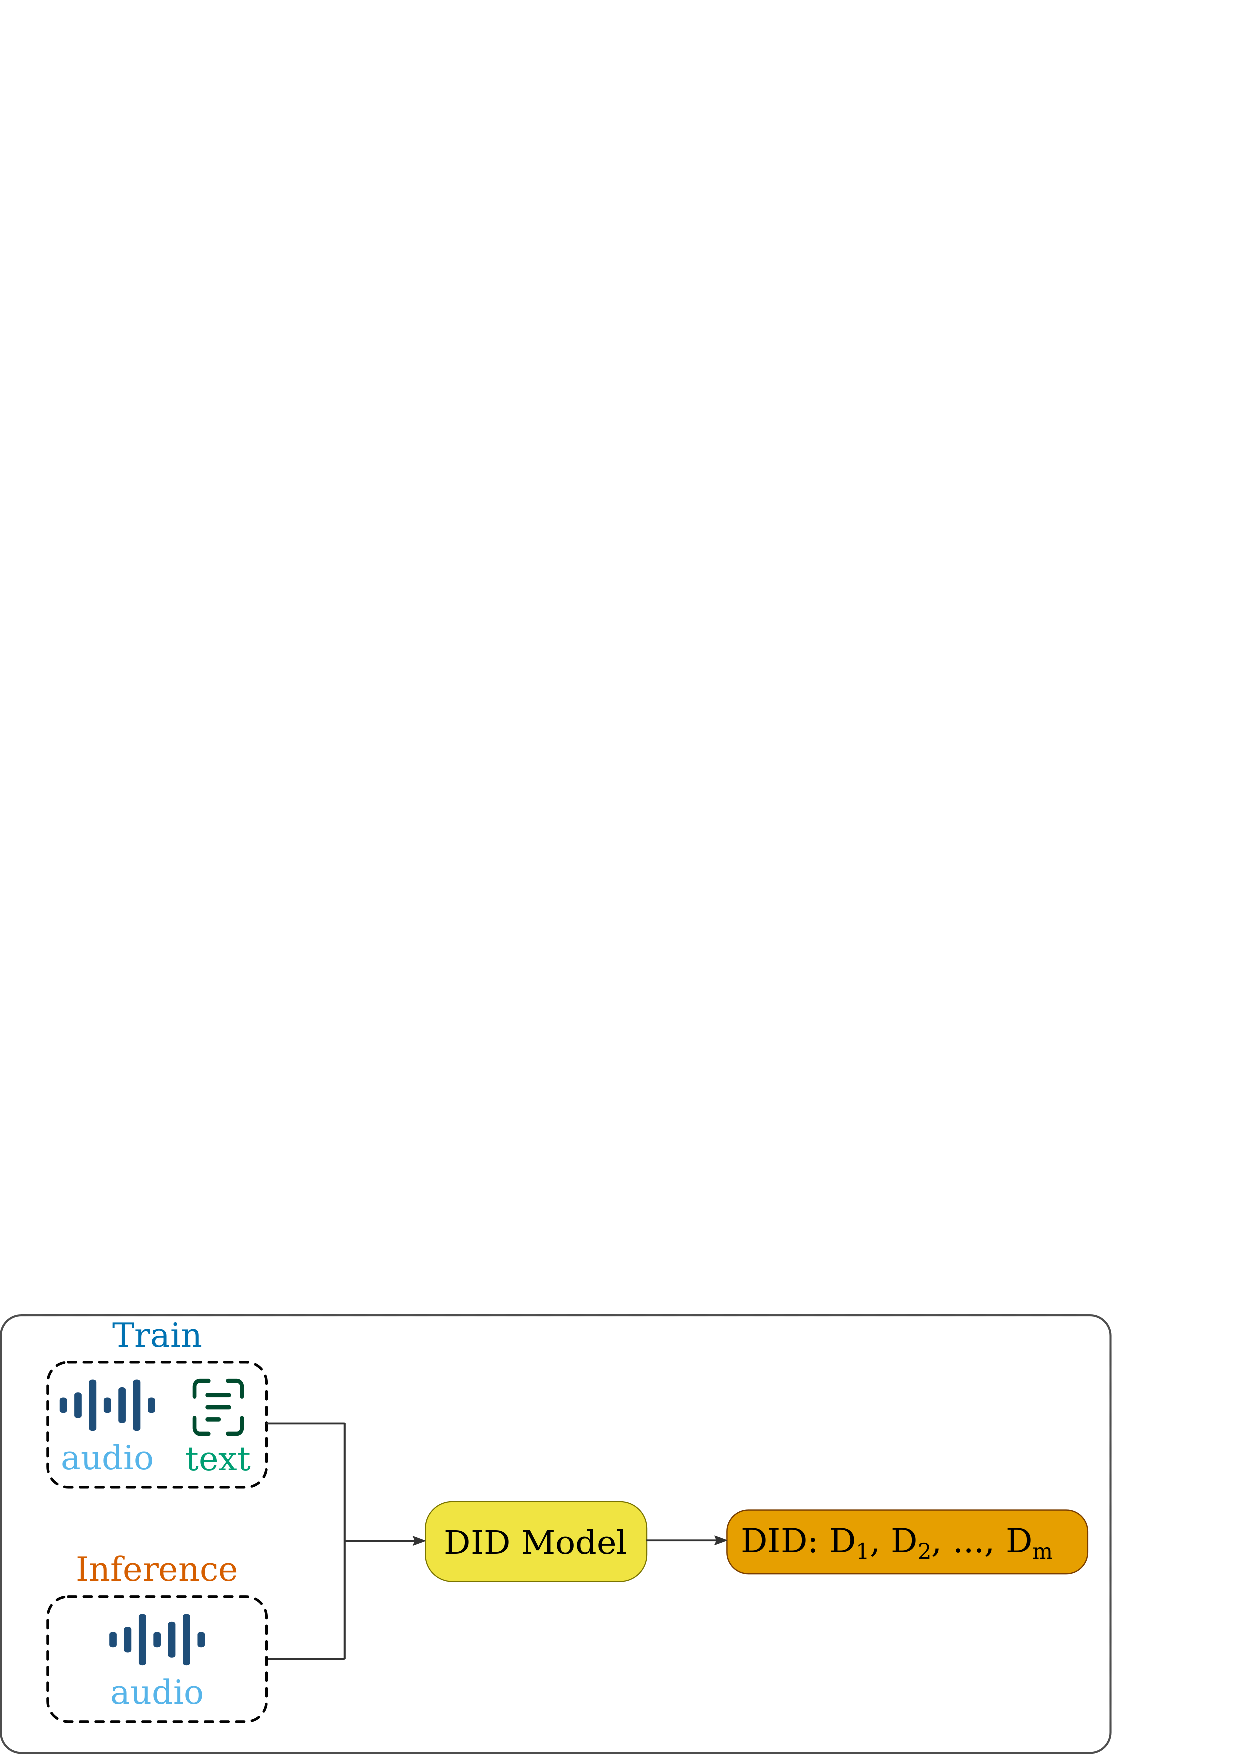
\includegraphics[width=0.8\textwidth]{presentation/Images/did_modalities.png}
  \end{minipage}

  % -------- RIGHT: 40% width (all text) --------
  \column{0.5\textwidth}
  \vspace{-3mm}
  \begin{minipage}[t]{\linewidth}
    \footnotesize
    \textbf{Key insight:}
    \begin{itemize}\itemsep2pt
      \item \textbf{Audio-only / Text-only} are \emph{suboptimal}: they fail to use complementary acoustic/lexical cues. In our prior work \cite{ICASSP25_DID}, these underperformed \emph{ASR-based DID} trained with \textbf{Audio+Text}.
      \item \textbf{Audio+Text (Train \& Test)} is \emph{limited in practice}: many under-resourced Indian languages lack transcribed data.
    \end{itemize}

    \textbf{Focus in this work:}
    \begin{itemize}\itemsep2pt
      \item \textbf{Train:} use \textbf{Audio+Text} to learn richer, complementary representations.
      \item \textbf{Test:} require \textbf{Audio-only} to enable scalable, transcript-free deployment.
    \end{itemize}
  \end{minipage}

\end{columns}

\end{frame}

\begin{frame}{The Problem: A Performance Trade-Off}
    \begin{itemize}
        \item Joint ASR--DID models often face a trade-off: gains in one task can degrade the other.
        
        \item \textbf{Prior findings:}
        \begin{itemize}
            \item Japanese: best DID setup degraded ASR performance \cite{Imaizumi_Japanese_DID2022}.
            \item Irish: improved DID slightly reduced ASR performance \cite{lonergan2024low}.
            \item Indian (8 langs.): multimodal features boosted DID but slightly degraded ASR \cite{ICASSP25_DID}.
        \end{itemize}

        \item \textbf{Common issue:}  
        Most ASR-based DID methods prepend/append dialect ID to training text. This false context significantly degrades ASR performance.

        \item \textbf{Our goal:}  
        Use dialect information as \emph{probabilistic features}, and improve \textbf{both} ASR and DID.
    \end{itemize}
\end{frame}

\begin{frame}{Our Contributions}
    \begin{itemize}
        \item A \textbf{novel joint framework} that improves both ASR and DID by fusing features with a gating mechanism:
        \begin{itemize}
            \item \textbf{Speech Features:} A Bottleneck Encoder~\cite{Srinivas_bneck_2021} refines Conformer outputs.
            \item \textbf{Text Features:} A RoBERTa encoder~\cite{Liu2019RoBERTaAR} processes ASR-generated CTC embeddings.
        \end{itemize}

        \item The fused dialect embedding enhances the ASR encoder directly, an approach that avoids prepending dialect tokens and improves robustness against DID errors.

        \item Achieved state-of-the-art results on \textbf{8 Indian languages} (33 dialects): \textbf{81.63\%} DID accuracy, \textbf{4.65\%} CER, and \textbf{17.73\%} WER.
        
        \item Publicly released code and models to encourage further research~\footnote{\url{https://github.com/labspire/respin_did_interspeech25.git}}.
    \end{itemize}
\end{frame}

%------------------------------------------------------------
% Proposed Method Section
%------------------------------------------------------------
\begin{frame}{Proposed Method: ASR-BN-ROB Architecture}

\begin{columns}[T]
    \column{0.30\textwidth}
        \centering
        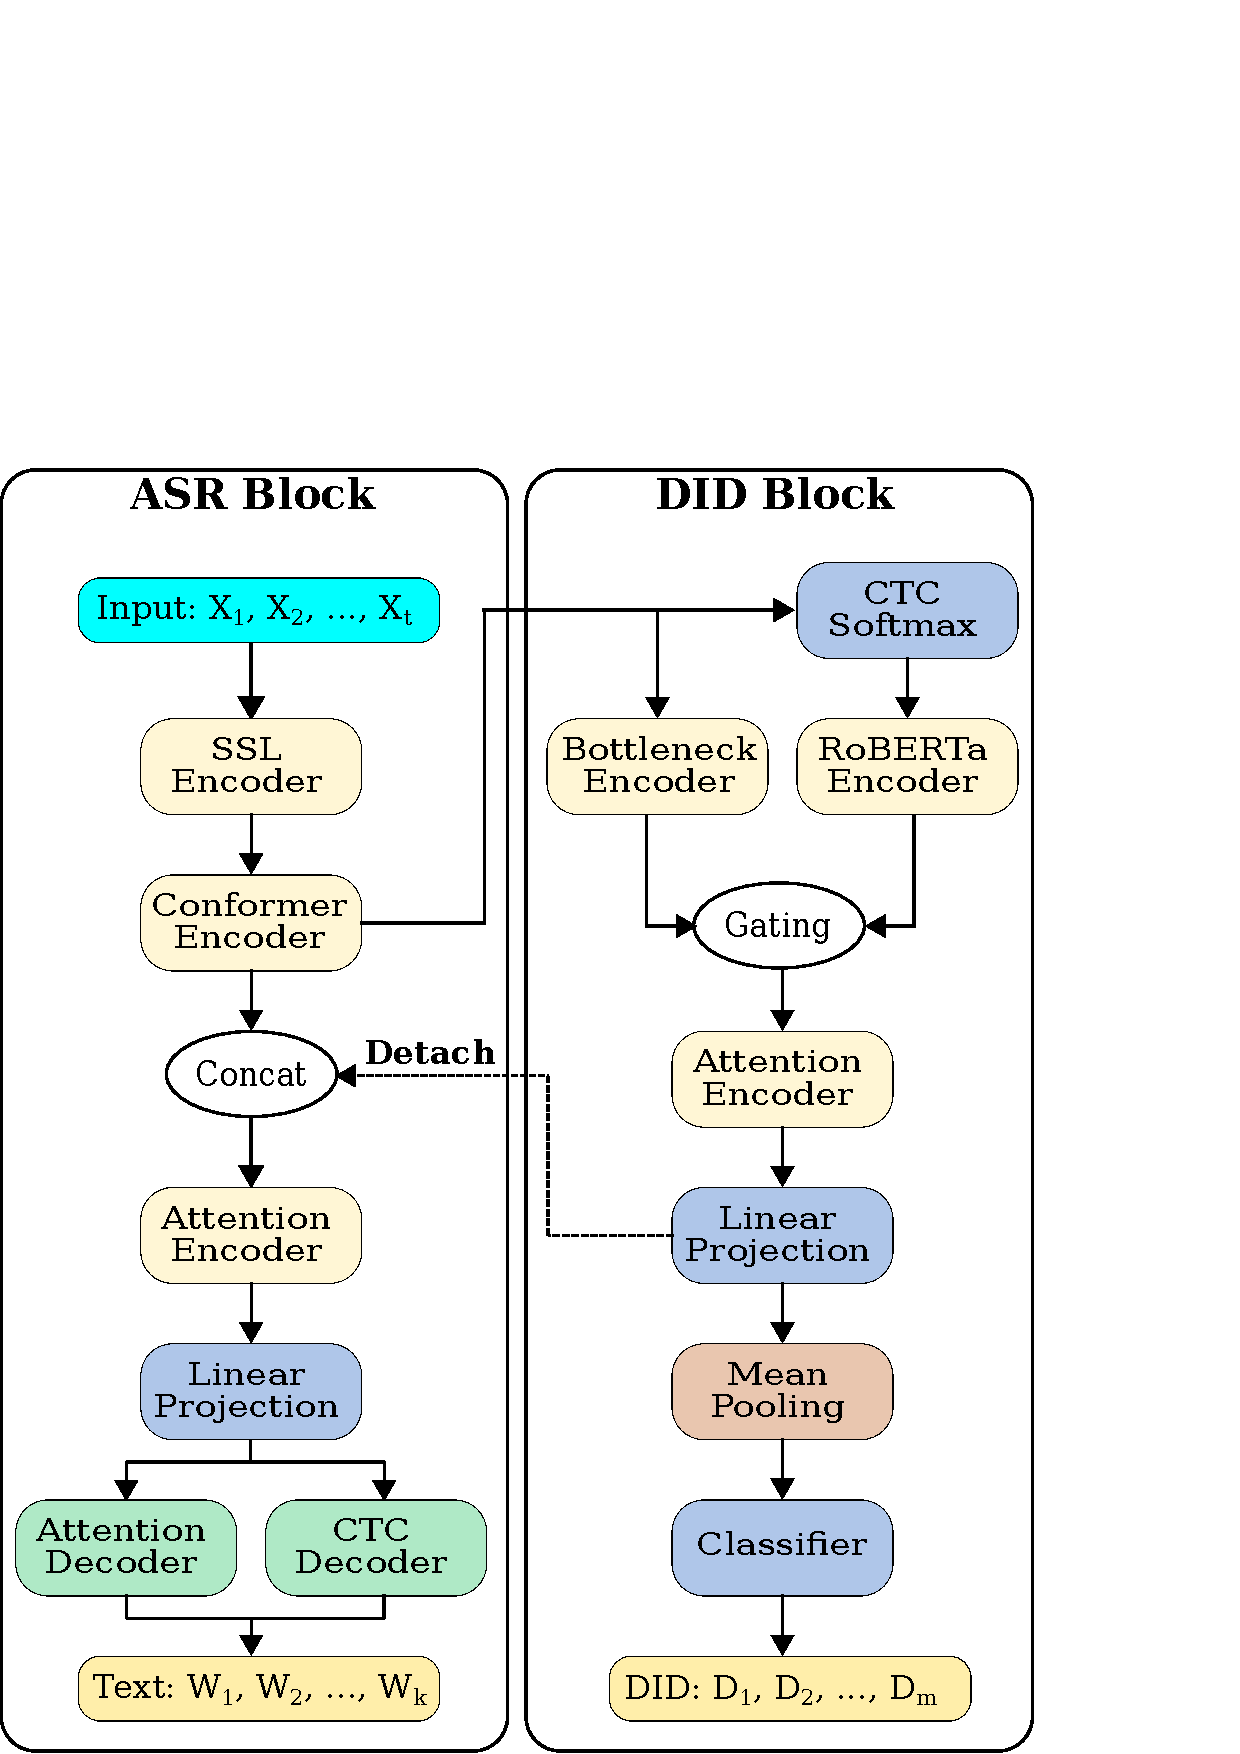
\includegraphics[height=0.75\textheight, keepaspectratio]{presentation/Images/asr_did_v3.pdf}

    \column{0.7\textwidth}
        \footnotesize
        \begin{itemize}
            \item \textbf{ASR-BN-ROB:} Joint ASR--DID using Bottleneck (BN) \cite{Srinivas_bneck_2021} encoder for speech features and RoBERTa (ROB) \cite{Liu2019RoBERTaAR} encoder for text features.
            \item \textbf{ASR Block:} Conformer-based CTC+Attention ASR with SSL features.
            \item \textbf{DID Block:} BN captures acoustic/temporal cues from ASR output; ROB processes CTC embeddings for lexical/semantic cues.
            \item \textbf{Fusion:} Gating mechanism adaptively combines BN and ROB features.
            \item \textbf{Integration:} Fused probabilistic dialect features fed back into ASR encoder (not as tokens) to avoid degradation from DID errors.
            \item \textbf{Stability:} Gradient detachment from DID to ASR ensures stable joint training.
        \end{itemize}
\end{columns}

\end{frame}

\begin{frame}{Bottleneck and Attention Encoder Architecture}

\begin{columns}[T]
    \column{0.3\textwidth}
        \centering
        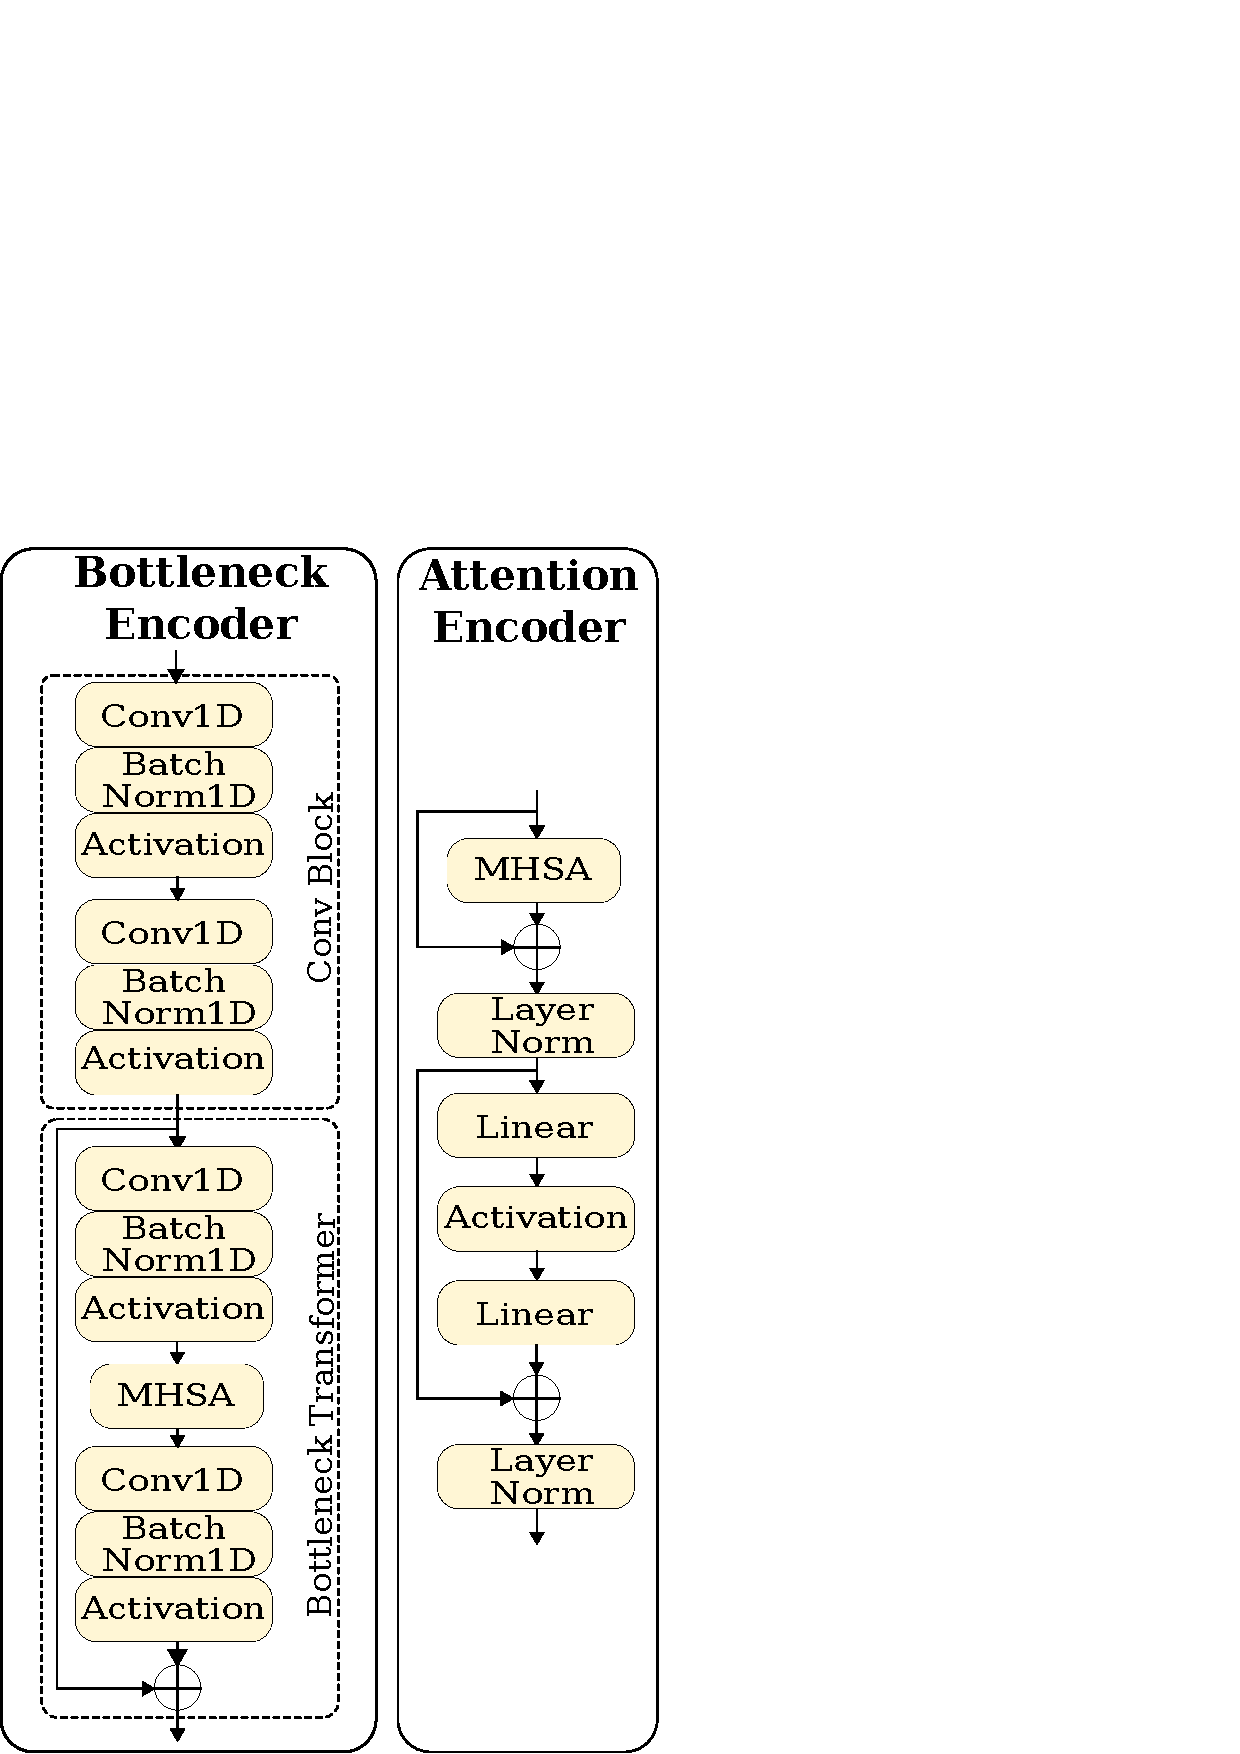
\includegraphics[height=0.75\textheight, keepaspectratio]{presentation/Images/bneck_enc.pdf}
        \vfill
        % \tiny \textbf{Figure:} Bottleneck and Attention Encoder architectures.

    \column{0.7\textwidth}
        \small
        \textbf{Bottleneck Encoder:}
        \begin{itemize}
            \item Extracts dialectal cues from Conformer output.
            \item Uses stacked Conv1D, BatchNorm, activations; MHSA further captures long-range context.
            \item Based on~\cite{Srinivas_bneck_2021}, with 1D convs and no pooling to preserve temporal info.
        \end{itemize}

        \vspace{0.3em}
        \textbf{Attention Encoder:}
        \begin{itemize}
            \item Refines fused speech-text features using MHSA, LayerNorm, residual FFN with up/down projections.
            \item Outputs frame-level embeddings; mean pooled for DID classification.
        \end{itemize}
\end{columns}

\end{frame}

\begin{frame}{DID Block: Gating and Attention Fusion}

\begin{columns}[T,onlytextwidth]
  \column{0.56\textwidth}
  \textbf{Gating:}
  \[
    \mathbf{G}=\sigma\!\big(\mathbf{W}_g[\mathbf{H}_{\text{bottleneck}},\mathbf{H}_{\text{rob}}]+\mathbf{b}_g\big)
  \]

  \medskip
  \textbf{Fusion:}
  \[
    \mathbf{H}_{\text{fused}}
    = \mathbf{G}\odot\mathbf{H}_{\text{rob}}
    + (1{-}\mathbf{G})\odot\mathbf{H}_{\text{bottleneck}}
  \]

  \medskip
  \textbf{Refinement:}
  \[
    \mathbf{H}_{\text{fused}} \xrightarrow{\ \text{Attention Encoder}\ } \text{Dialect embedding}
  \]

  \column{0.44\textwidth}
  \small
  \textbf{Notes:}
  \begin{itemize}\itemsep2pt
    \item $\mathbf{H}_{\text{bottleneck}}$: BN (speech) features
    \item $\mathbf{H}_{\text{rob}}$: ROB (text) features from CTC embeddings
    \item $[\cdot,\cdot]$: concat along feature dim
    \item $\mathbf{W}_g,\mathbf{b}_g$: learnable weights, bias
    \item $\sigma(\cdot)$: element-wise sigmoid
    \item $\odot$: element-wise multiplication
  \end{itemize}
\end{columns}

\end{frame}



\begin{frame}{Joint Optimization Objective}

\textbf{Goal:} Train ASR and DID jointly using a multi-task loss.

\vspace{0.5em}
\textbf{Total Loss:}
\[
L = \underbrace{\lambda_{CTC} \mathcal{L}_{CTC} + (1 - \lambda_{CTC}) \mathcal{L}_{ATT}}_{\text{ASR Loss}} + \underbrace{\gamma_{CE} \mathcal{L}_{CE}}_{\text{DID Loss}}
\]

\begin{itemize}
    \item $\mathcal{L}_{CTC}$: CTC loss for faster convergence and alignment.
    \item $\mathcal{L}_{ATT}$: Attention decoder loss for richer context modeling.
    \item $\mathcal{L}_{CE}$: Cross-entropy loss for dialect classification.
    \item $\lambda_{CTC}$, $\gamma_{CE}$: Control ASR-DID loss balance.
\end{itemize}

\end{frame}

%------------------------------------------------------------
% Experiments Section
%------------------------------------------------------------
\section{Experiments and Setup}

\begin{frame}{Experimental Setup: Dataset}
    \textbf{Dataset}
    \begin{itemize}
        \item We use a subset of the \textbf{RESPIN}~\cite{respin} dataset, following the same data split as in~\cite{ICASSP25_DID}.
        \item Covers \textbf{8 Indian languages}:
        \begin{itemize}
            \item Bhojpuri (bh), Bengali (bn), Chhattisgarhi (ch), Kannada (kn), Magahi (mg), Maithili (mt), Marathi (mr), and Telugu (te).
        \end{itemize}
        \item A total of \textbf{33 distinct dialects} across these languages.
        \item Approximately 140-175 hours of training data in a read-speech setting.
    \end{itemize}

    \begin{table}[h]
    \centering
    \small
    \begin{tabular}{lcccccccc}
    \toprule
    \textbf{Lang} & bh & bn & ch & kn & mg & mr & mt & te \\
    \midrule
    \textbf{\#Dialects} & 3 & 5 & 4 & 5 & 4 & 4 & 4 & 4 \\
    \bottomrule
    \end{tabular}
    \caption{Number of dialects per language in the RESPIN dataset.}
    \end{table}

\end{frame}

\begin{frame}{Dataset: Preserving Dialect in Read-Speech}
\begin{columns}[T]
    % -------- LEFT COLUMN --------
    \column{0.7\textwidth}
    \vspace{-2mm}
    \begin{itemize}
      \item \textbf{All RESPIN data in this work are read-speech.}
      \item \textbf{Design to preserve dialectal diversity:}
      \begin{itemize}
        \item \textit{Sentence composition:} Native composers wrote in regional/colloquial variants.
        \item \textit{No normalization:} No orthographic or lexical standardization at composition time.
        \item \textit{Speaker selection:} Native speakers from the corresponding dialect regions.
        \item \textit{Reading protocol:} Speakers read \emph{exactly as written}, without normalization or “standard” correction.
      \end{itemize}
      \item \textbf{Outcome:} Dialect-specific lexical, phonetic, and syntactic cues are preserved in both text and audio, despite the read-speech setting.
    \end{itemize}

    % -------- RIGHT COLUMN --------
    \column{0.3\textwidth}
    \centering
    \vspace{-2mm}
    \textbf{Examples \& Code} \\
    % \vspace{2mm}
    \url{https://github.com/labspire/respin_did_interspeech25} \\
    % \vspace{3mm}
    \includegraphics[width=0.8\textwidth]{presentation/Images/git_repo_qr.png} \\
    {\scriptsize Scan for audio \& text examples}
\end{columns}
\end{frame}


\begin{frame}{Experimental Setup: Baselines}
    \textbf{Compared Methods}
    \begin{itemize}
        \item \textbf{Base-ASR:} Conformer-based CTC+Attention ASR (SSL features), no DID component.
        \item \textbf{ASR-DID:} Ground-truth dialect ID prepended to training text.
        \item \textbf{ASR-DID-AUX:} ASR-DID with auxiliary CTC loss for DID.
        \item \textbf{ASR-DID-ROB (baseline):} Uses RoBERTa encoder on CTC embeddings for DID. 
        \begin{itemize}
            \item Chosen as baseline because in our recent work \cite{ICASSP25_DID}, 
            it outperformed other ASR-DID variants in terms of DID accuracy.
        \end{itemize}
        \item \textbf{Proposed: ASR-BN-ROB} and ablations:
        \begin{itemize}
            \item \textbf{ASR-BN:} Bottleneck encoder only (speech features).
            \item \textbf{ASR-ROB:} RoBERTa encoder only (text features).
        \end{itemize}
    \end{itemize}
\end{frame}


%------------------------------------------------------------
% Results Section
%------------------------------------------------------------
\section{Results}

\begin{frame}{DID Performance: Accuracy (\%)}
    \begin{table}
        \centering
        \caption{Our proposed model achieves the highest average DID accuracy.}
        \resizebox{0.7\textwidth}{!}{%
        \begin{tabular}{lccccccccc}
            \toprule
            \textbf{System} & \textbf{bh} & \textbf{bn} & \textbf{ch} & \textbf{kn} & \textbf{mg} & \textbf{mr} & \textbf{mt} & \textbf{te} & \textbf{Avg} \\
            \midrule
            ASR-DID         & 74.91 & 72.43 & 77.81 & 80.08 & 86.26 & 82.07 & 82.35 & 77.58 & 79.19 \\
            ASR-DID-SC      & 75.54 & 72.64 & 76.60 & 80.96 & 86.19 & 82.72 & 81.94 & 78.89 & 79.44 \\
            ASR-DID-AUX     & 75.72 & 73.10 & 76.38 & 81.80 & 86.88 & 81.64 & 82.77 & 80.28 & 79.82 \\
            ASR-DID-ROB (baseline) & 77.43 & 73.38 & 77.00 & 83.18 & 87.31 & 82.90 & 83.67 & 81.06 & 80.74 \\
            \midrule
            ASR-ROB         & 77.32 & 74.28 & 76.33 & 83.11 & 87.77 & 83.18 & 83.62 & 79.22 & 80.60 \\
            ASR-BN          & 77.39 & 73.19 & 78.88 & 82.56 & 87.59 & 81.82 & \textbf{84.22} & 80.82 & 80.81 \\
            \textbf{ASR-BN-ROB (Proposed)} & \textbf{78.74} & \textbf{74.46} & \textbf{79.38} & \textbf{83.55} & \textbf{87.88} & \textbf{83.66} & 83.11 & \textbf{82.23} & \textbf{81.63} \\
            \bottomrule
        \end{tabular}
        }
    \end{table}
    \begin{itemize}
        \item The proposed ASR-BN-ROB model, which fuses both modalities, achieves the highest average DID accuracy of \textbf{81.63\%}.
        \item This demonstrates the benefit of multimodal fusion over single-modality approaches.
    \end{itemize}
\end{frame}


\begin{frame}{DID Confusion Matrices: Baseline vs. Proposed}
    \begin{columns}[c]
        \column{0.5\textwidth}
            \centering
            \includegraphics[width=\textwidth]{presentation/Images/baseline_confusion_matrices.pdf} \\
            \tiny (a) Baseline (ASR-DID-ROB)
        
        \column{0.5\textwidth}
            \centering
            \includegraphics[width=\textwidth]{presentation/Images/proposed_confusion_matrices.pdf} \\
            \tiny (b) Proposed (ASR-BN-ROB)
    \end{columns}
    % \vspace{0.5cm}
    \begin{itemize}
        \item \textbf{Key Insight:} Our model not only improves overall accuracy but also enhances generalization across dialects.
        \item This is shown by a \textbf{16.08\% average reduction} in the standard deviation of dialect-wise accuracies, indicating more consistent and robust performance.
    \end{itemize}
\end{frame}

\begin{frame}{ASR Performance: CER (\%) and WER (\%)}
    \vspace{-5mm}
    \begin{table}
        \centering
        \caption{Proposed method improves ASR while also boosting DID.}
        \resizebox{0.7\textwidth}{!}{%
        \begin{tabular}{l|cc|cc}
            \toprule
            & \multicolumn{2}{c|}{\textbf{Average CER (\%)}} & \multicolumn{2}{c}{\textbf{Average WER (\%)}} \\
            \textbf{System} & \textbf{CER} & \textbf{Rel. Impr.} & \textbf{WER} & \textbf{Rel. Impr.} \\
            \midrule
            Base-ASR                  & 4.81 & --    & 18.38 & --    \\
            ASR-DID-ROB (baseline) & 4.76 & 1.0\%  & 18.16 & 1.2\%  \\
            \midrule
            \textbf{ASR-BN-ROB (proposed)} & \textbf{4.65} & \textbf{3.3\%} & \textbf{17.73} & \textbf{3.5\%} \\
            \bottomrule
        \end{tabular}
        }
    \end{table}
    \vspace{-1mm}
    \begin{itemize}
        \item \textbf{Best ASR performance:} CER 4.65\%, WER 17.73\%.
        \item \textbf{Breaks the trade-off:} Previous joint methods often degraded ASR, but our model improves both ASR and DID.
        \item Full language-wise results are reported in the paper.
    \end{itemize}
\end{frame}

\begin{frame}{Analysis: Impact of Incorrect DID on ASR}
    \begin{itemize}
        \item A key challenge for some joint models is their reliance on prepending dialect IDs to text.
        \item \textbf{What happens when the DID prediction is wrong?}
        \begin{itemize}
            \item The ASR model is conditioned on "false context".
            \item This can significantly harm transcription accuracy, worsening the ASR/DID trade-off.
        \end{itemize}
        \item We analyse ASR performance specifically on utterances where the baseline model misclassifies the dialect.
        \item \textbf{Hypothesis:} Our model, which does not prepend IDs, should be more robust to these errors.
    \end{itemize}
\end{frame}

\begin{frame}{Analysis: ASR Robustness to DID Errors}
    \vspace{-7mm}
    \begin{table}
        \centering
        \caption{ASR performance on utterances with correct vs. incorrect DID predictions.}
        \resizebox{0.7\textwidth}{!}{%
        \begin{tabular}{l|cc|cc}
            \toprule
            & \multicolumn{2}{c|}{\textbf{CER (\%)}} & \multicolumn{2}{c}{\textbf{WER (\%)}} \\
            \textbf{ASR System} & \textbf{Incorrect} & \textbf{Correct} & \textbf{Incorrect} & \textbf{Correct} \\
            \midrule
            Base-ASR & 5.67 & 4.66 & 20.74 & 17.93 \\
            ASR-DID-ROB (baseline) & 6.01 & 4.51 & 21.85 & 17.43 \\
            \textbf{ASR-BN-ROB (proposed)} & \textbf{5.68} & \textbf{4.46} & \textbf{20.72} & \textbf{17.14} \\
            \midrule
            \textbf{Relative difference (\%)} & \textbf{5.52} & 1.24 & \textbf{5.17} & 1.62 \\
            \bottomrule
        \end{tabular}
        }
    \end{table}
    
    \vspace{-2mm}
    \begin{itemize}
        \item \textbf{Key takeaway:} Proposed model is more robust, especially when DID is incorrect.
        \item \textbf{Incorrect DID:} \textbf{5.52\% CER} and \textbf{5.17\% WER} relative reduction over baseline.
        \item \textbf{Correct DID:} Consistent small gains in both CER and WER.
    \end{itemize}
\end{frame}


\begin{frame}{Language-wise CER for Incorrect vs Correct DID predictions}

\begin{columns}[T]
    \column{0.7\textwidth}
    \centering
    \includegraphics[width=\textwidth]{presentation/Images/language_wise_cer_bar_plot.png}

    \column{0.3\textwidth}
    \small
    \textbf{Observations:}
    \begin{itemize}
        \item CER is consistently lower when DID predictions are correct.
        \item ASR-BN-ROB yields the lowest CER across most languages.
        \item Compared to ASR-DID, largest CER improvement observed in \textbf{mt}, \textbf{te}, and \textbf{ch} for incorrect DID.
    \end{itemize}
\end{columns}

\end{frame}


\begin{frame}{Statistical Significance}
    \begin{itemize}
        \item To confirm the robustness of our results, we performed a paired T-test at a 95\% confidence interval across the 8 languages, comparing our proposed model to the ASR-DID-ROB baseline.
        \item The improvements are \textbf{statistically significant} for all key metrics:
        \begin{itemize}
            \item \textbf{DID Accuracy:} $p = 0.0211$
            \item \textbf{ASR CER:} $p = 0.0002$
            \item \textbf{ASR WER:} $p = 0.0006$
        \end{itemize}
        \item These results strongly validate the effectiveness of our proposed multimodal fusion approach.
    \end{itemize}
\end{frame}

%------------------------------------------------------------
% Conclusion Section
%------------------------------------------------------------
\section{Conclusion}

\begin{frame}{Conclusion}
    \begin{itemize}
        \item We presented a novel multimodal feature fusion approach that successfully improves both DID and ASR for Indian languages, mitigating the traditional performance trade-off.
        \item By integrating speech features (Bottleneck Encoder) and text features (RoBERTa on CTC embeddings) through an adaptive gating mechanism, our model achieves superior performance.
        \item Our proposed ASR-BN-ROB model establishes a new state-of-the-art, with \textbf{81.63\% DID accuracy}, \textbf{4.65\% CER}, and \textbf{17.73\% WER}.
        \item The model is also more robust to incorrect dialect predictions, a key weakness in previous systems.
    \end{itemize}
\end{frame}

\begin{frame}{Future Work}

\begin{itemize}
    \item \textbf{Expand to spontaneous and real-world speech:}
    \begin{itemize}
        \item Evaluate the fusion approach on spontaneous, conversational, and noisy speech scenarios.
        \item Extend to multilingual and code-switched ASR settings.
    \end{itemize}
    
    \item \textbf{Generalize across dialects and languages:}
    \begin{itemize}
        \item Assess model robustness across a wider set of dialects and under-represented languages.
    \end{itemize}

    \item \textbf{Explore learning paradigms:}
    \begin{itemize}
        \item Investigate unsupervised and semi-supervised techniques to reduce label dependence.
        \item Study alternative fusion strategies and upstream SSL feature encoders.
    \end{itemize}
\end{itemize}

\end{frame}

%------------------------------------------------------------
% References Section
%------------------------------------------------------------
\section{References}
\footnotesize
\begin{frame}[allowframebreaks]{References}
    \bibliographystyle{apalike}
    \bibliography{refs}
\end{frame}


%------------------------------------------------------------
% Acknowledgements & Thank You
%------------------------------------------------------------
\begin{frame}{Acknowledgments}
    \begin{itemize}
        \item This work was supported by the \textbf{RESPIN project}, funded by the Gates Foundation.
        \item We extend our thanks to the entire RESPIN team and our project partner, Navana Tech, for their valuable contributions to data collection.
    \end{itemize}
\end{frame}

\begin{frame}
    \vfill
    \centering
    {\Huge \textbf{Thank You!}} \\
    \vspace{2mm}
    {\Large Questions or Suggestions?} \\
    \vspace{4mm}

    \begin{columns}[T,totalwidth=\textwidth]
        % Right column: QR code
        \column{0.45\textwidth}
        \centering
        \includegraphics[height=0.6\textheight, keepaspectratio]{presentation/Images/git_repo_qr.png} \\%[2mm]
        {\small Scan for code and resources}

        % Left column: Contact & Links
        \column{0.55\textwidth}
        \small
        % \raggedright
        \textbf{Code Repository:} \\
        \href{https://github.com/labspire/respin_did_interspeech25}{\texttt{github.com/labspire/respin\_did\_interspeech25}} \\[3mm]
        
        \textbf{Contact:} \\
        \href{mailto:saurabhk0317@gmail.com}{\texttt{saurabhk0317@gmail.com}} \\
        \href{mailto:spirelab.ee@iisc.ac.in}{\texttt{spirelab.ee@iisc.ac.in}} \\
    \end{columns}

    \vfill
\end{frame}

% \begin{frame}[t]{SPIRE Open-Source Datasets}
% % \framesubtitle{Speech & Language resources from SPIRE Lab, IISc Bangalore}

% \begin{columns}[T, totalwidth=\textwidth]
%     % Left column: image
%     \begin{column}{0.65\textwidth}\vspace{-4mm}
%         \includegraphics[height=0.85\textheight, keepaspectratio]{presentation/Images/spire_datasets.jpeg}
%     \end{column}

%     % Right column: short note + link
%     \begin{column}{0.35\textwidth}
%         \vfill
%         {\small\itshape 
%         All datasets are accessible via the QR code in the figure.\\[3mm]
%         \textbf{Scan to explore!}\\[5mm]
%         \href{https://spiredatasets.ee.iisc.ac.in/}{\texttt{spiredatasets.ee.iisc.ac.in}}}
%         \vfill
%     \end{column}
% \end{columns}

% \end{frame}

\begin{frame}[t]{SPIRE Open-Source Datasets}
    \vspace{-2mm}
    \centering
    \includegraphics[height=0.75\textheight, keepaspectratio]{presentation/Images/spire_datasets_189.pdf}
    
    % \vspace{0.3cm}
    \small Scan the QR code or visit 
    \textbf{\textit{\href{https://spiredatasets.ee.iisc.ac.in/}{spiredatasets.ee.iisc.ac.in}}} for more details.
\end{frame}

\end{document}

